\documentclass[a4paper, 10pt]{article}

\usepackage{tabularx} % extra features for tabular environment
\usepackage{amsmath}  % improve math presentation
\usepackage{graphicx} % takes care of graphic including machinery
\usepackage[margin=1in,letterpaper]{geometry} % decreases margins
\usepackage{cite} % takes care of citations
\usepackage[final]{hyperref} % adds hyper links inside the generated pdf file
\usepackage{ctex}
\usepackage{titlesec}
%\usepackage{CJKutf8, CJK}
\usepackage{makecell}                 % 三线表-竖线
\usepackage{booktabs}                 % 三线表-短细横线
% \usepackage{natbib}
\usepackage{graphicx}				  % 表格单元格逆时针
\usepackage{multirow}				  % 合并单元格
\usepackage{array}
\usepackage{amssymb}				  % 勾
\usepackage{amsmath}
\usepackage{longtable}                % 导入 longtable 宏包,表格自动换行
\usepackage{caption}
\usepackage{subcaption}               % 设置子图
\usepackage{color}					  % 文本颜色包
\usepackage{xcolor}
\usepackage{bbm}					  % 输入指示函数
\usepackage{tablefootnote}			  % 表格注释
\usepackage{pythonhighlight}
\usepackage{fancyhdr}
\usepackage{lastpage}
\usepackage{tocloft}
\pagestyle{fancy}
\fancyhf{}
\fancyhead{}
\fancyfoot{}
\fancyhead[R]{\small Page \thepage\ of \pageref*{LastPage}}
\fancyhead[L]{\small Report}

\usepackage{listings}                 % 导入代码块
\usepackage{xcolor}
\lstset{
	numbers=left, 
	tabsize=1,
	columns=flexible, 
	numberstyle=  \small, 
	keywordstyle= \color{ blue!70},
	commentstyle= \color{red!50!green!50!blue!50}, 
	frame=shadowbox, % 阴影效果
	rulesepcolor= \color{ red!20!green!20!blue!20} ,
	escapeinside=``, % 英文分号中可写入中文
	xleftmargin=2em,
	xrightmargin=2em, 
	aboveskip=1em,
} 

\hypersetup{
	colorlinks=true,       % false: boxed links; true: colored links
	linkcolor=blue,        % color of internal links
	citecolor=blue,        % color of links to bibliography
	filecolor=magenta,     % color of file links
	urlcolor=blue         
}
%++++++++++++++++++++++++++++++++++++++++
\titleformat{\section}{\Large\bfseries\songti}{\thesection}{1em}{}
\titleformat{\subsection}{\large\bfseries\songti}{\thesubsection}{1em}{}
\titleformat{\subsubsection}{\normalsize\bfseries\songti}{\thesubsubsection}{1em}{}
\titleformat{\paragraph}{\small\bfseries\songti}{\paragraph}{1em}{}
\titleformat{\subparagraph}{\footnotesize\bfseries\songti}{\subparagraph}{1em}{}

\begin{document}
	
	
	\title{\songti \zihao{4}3月工作汇报}
	\author{\textrm{Ku Jui}}
	\date{\textrm{March 2024}}
	\maketitle
	
	\renewcommand{\figurename}{Figure} % 可以重新定义abstract,因为ctex会覆盖thebibliography
	% 	\begin{abstract}
		%		In this experiment we studied a very important physical effect by measuring the
		%		dependence of a quantity $V$ of the quantity $X$ for two different sample
		%		temperatures.  Our experimental measurements confirmed the quadratic dependence
		%		$V = kX^2$ predicted by Someone's first law. The value of the mystery parameter
		%		$k = 15.4\pm 0.5$~s was extracted from the fit. This value is
		%		not consistent with the theoretically predicted $k_{theory}=17.34$~s. We attribute %this
		%		discrepancy to low efficiency of our $V$-detector.
		%	\end{abstract}
	
	\renewcommand{\tablename}{Table}
	
	% 设置目录标题为居中
	\renewcommand{\cfttoctitlefont}{\hfill\Large\bfseries\songti}
	\renewcommand{\cftaftertoctitle}{\hfill}
	\renewcommand{\contentsname}{Content}
		
	\tableofcontents
	
	\newpage	
	
	\section{引言}
		
		低光图像增强(Low-Light Image Enhancement, LLIE)是图像处理领域的一个关键任务,旨在提升低光环境下拍摄图像的视觉质量。该领域的最新进展主要由深度学习技术推动,包括多种学习策略、网络架构、损失函数和训练数据集的应用。低光图像增强在视觉监控、自动驾驶和计算摄影等多个领域具有广泛应用。尤其在智能手机摄影领域,由于相机光圈大小、实时处理需求和存储限制,低光环境下的图像拍摄面临着显著挑战。
		
		%介绍传统的低光图像增强方法
		传统的低光增强方法,如基于直方图均衡化\cite{ji1994adaptive}和Retinex理论\cite{land1965, land1977retinex, jobson1997properties}的方法,虽然能够在一定程度上改善图像质量,但存在一些局限性。直方图均衡化能够提高图像的全局对比度,但可能增加背景噪声的对比度并降低有用图像内容的对比度,导致视觉效果不佳。Retinex算法旨在消除图像照度分量的干扰并还原图像真实色彩,但通常忽略噪声问题,可能导致增强结果中噪声的保留或放大,并且其复杂的优化过程增加了模型的复杂度。
		
		%传统的低光增强方法,如基于直方图均衡\cite{ji1994adaptive}和 Retinex\cite{land1965, land1977retinex, jobson1997properties}的方法,直方图均衡化重新调整图像的直方图分布,一方面增加了图像的全局对比度,另一方面使得亮度在整个图像的分布更加均匀。直方图均衡化的方法非常快速有效,并且是一个可逆操作,但缺点在于其不加选择地处理数据,可能增加背景噪声的对比度,同时降低有用的图像内容的对比度,导致视觉效果欠佳。此外,该方法也无法适用于复杂多变的低光照场景。Retinex 算法的核心思想是消除源图像照度分量干扰,依据反射分量信息还原图像真实色彩。基于 Retinex 的方法能够很大程度改善图像质量,但在应用的过程中仍存在不可忽视的缺点。例如,其通常忽略噪声问题,可能导致增强结果中噪声的保留或放大;有效的先验或正则化的选择具有挑战性,不准确的先验可能导致伪影和颜色偏差;此外,这些方法的复杂优化过程也导致最终的模型较为复杂。
		
		近年来,基于深度学习的低光图像增强技术取得了显著成就,特别是卷积神经网络(CNN)在多个计算机视觉任务中展现出卓越的性能。CNN通过利用注意力机制\cite{yang2021locally,zhang2020attention}和上下文信息,能够从原始图像中有效提取局部特征\cite{jain1991unsupervised, lowe2004distinctive, ojala2002multiresolution}。\textcolor{red}{在低光图像中,亮度较低、对比度较弱的区域之间存在一定的关联性和相互作用,如果模型能够捕获全局光照,将有助于恢复图像的整体亮度和对比度\cite{chen2018learning, wang2013naturalness}\footnote{Retinex 理论的一个关键思想是图像的颜色和亮度感知取决于全局光照条件,因此捕获和调整全局光照信息对于图像增强和恢复至关重要。}。在图像处理领域,尤其是在低光图像恢复和增强方面,保持图像的结构完整性是一个重要的挑战。Fu 等人\cite{fu2016weighted}引入了一种加权变分模型,通过边缘感知权重来保持图像的结构完整性,从而在增强过程中保持边缘和细节信息。随后,Wang 等人\cite{wang2018esrgan}在其提出的 ESRGAN 模型中强调了集成全局和局部特征的重要性,包括保持边缘和纹理细节的完整性,以增强图像的感知质量。最近,Xu\cite{xu2020learning}提出了一种基于深度学习的方法,通过分解和增强来恢复低光图像,其中在分解阶段保持了图像的结构信息,包括边缘和纹理细节,这对于后续的增强阶段至关重要。因此,即使在低光条件下,对象的轮廓和边缘仍然是重要的视觉特征,捕获这些长距离的边缘信息对于保持图像的结构完整性至关重要。}
		
		在低光条件下捕获和恢复图像中的纹理和模式是图像增强领域的一项重要挑战。\textcolor{red}{Loh等人\cite{loh2019getting}通过对低光照图像的特性进行研究,强调了在弱光条件下保持图像纹理和模式的重要性。进一步地,Jiang 等人\cite{jiang2021enlightengan}提出了一种基于生成对抗网络的方法,有效地恢复了低光图像中的细节,包括难以辨识的纹理和模式。同样,Lv 等人\cite{lv2018mbllen}通过卷积神经网络增强了低光图像和视频,专注于恢复纹理和模式的细节,从而提供更丰富的图像内容。因此,尽管弱光图像中的纹理和模式可能难以辨识,但它们对于理解图像内容仍然非常重要。理解图像内容的关键在于识别不同对象和场景元素之间的空间关系。Wei 等人\cite{wei2018deep}提出的深度 Retinex 分解方法通过在特征提取过程中考虑长距离依赖关系来进一步提高低光图像的质量。}
		
		\textcolor{red}{在低光图像增强领域,现有的基于 CNN 的方法面临着一些挑战。Hao等人\cite{hao2020low}提出了一种半解耦分解的方法来增强低光图像,该方法旨在解决局部光照不均匀的问题,并改善颜色和细节的恢复。他们指出,传统的基于 CNN 的方法可能无法有效处理这些问题。同样,Ravirathinam 等人\cite{ravirathinam2021c}提出了一种多上下文特征提取模块,该模块专注于捕获高级上下文特征、结构相似性和局部信息。他们的研究指出,仅依赖局部感受野的 CNN 方法可能难以充分利用全局上下文信息。此外,Xu等人\cite{xu2021novel}提出了一种多尺度特征引导的注意力机制,以更多地关注那些黑暗和信息丰富的区域。他们强调,单一尺度的 CNN 方法可能受到感受野大小的限制,导致在处理细节丢失和局部光照不均匀问题时效果不佳。因此,开发能够克服这些限制并有效提升低光图像质量的深度学习模型仍然是一个重要的研究方向。}
		
%		在低光图像中亮度较低、对比度较弱的区域之间存在一定的关联性和相互作用,如果模型能够捕获全局光照有助于恢复图像的整体亮度和对比度。
%		
%		同样,即使在低光条件下,对象的轮廓和边缘仍然是重要的视觉特征。捕获这些长距离的边缘信息对于保持图像的结构完整性至关重要。
%		
%		纹理和模式,低光图像中的纹理和模式可能难以辨识,但它们对于理解图像内容仍然很重要。长距离特征可以帮助模型识别和恢复这些纹理和模式。
%		
%		不同对象和场景元素之间的空间关系是理解图像的关键。在低光图像中,捕获这些长距离的上下文关系对于正确的解释图像至关重要。
%		
%		然而,现有的基于CNN的方法在处理局部光照不均匀、颜色信息和细节信息丢失问题时,仍存在过增强或增强不足的挑战,并且增强结果受到感受野大小的限制。


%		
		%近年来,基于深度学习的低光图像增强 (LLIE) 方法取得了显著的成功。与传统方法相比,基于深度学习的解决方案在准确性、鲁棒性和速度方面表现更佳,因此受到了越来越多的关注。近年来,基于深度学习的低光图像增强 (LLIE) 技术取得了显著成就,它使用神经网络来学习从弱光图像到自然光图像的映射。与传统方法相比,基于深度学习的解决方案在准确性、鲁棒性和处理速度方面表现更优,因此受到了广泛关注。特别是卷积神经网络(CNN)在多个计算机视觉任务中展现出卓越的性能。CNN 通过利用注意力机制和\cite{yang2021locally, zhang2020attention}上下文信息,能够从原始图像中有效提取多尺度特征\cite{li2018multi, zamir2020learning}。在这些成果的推动下,基于 CNN 的低光图像增强方法得到了持续发展。此外,现有的基于 CNN 的方法大多集中于图像亮度、纹理和颜色的恢复,对于局部光照不均匀、颜色信息和细节信息的丢失问题,仍存在过增强或增强不足的挑战,同时增强结果受到感受野大小的限制,但通过增大卷积核以及多次卷积的方法进行卷积又会增加模型的复杂度。
		
		为了解决这些问题,我们提出了一种新颖的方法(方法名待定)。受到ULite\cite{dinh20231m}中深度可分离卷积的启发,我们将U-Net网络中的卷积改为轴向深度可分离卷积,以减少模型冗余同时保持增强效果。此外,我们借鉴Swin-Unet\cite{cao2022swin}在BottleNeck中使用连续的Swin Transformer块以捕获图像长距离特征,相较于传统的Transformer块,Swin Transformer能够减少参数量和模型复杂度。通过以上改进,我们的方法能够有效提升低光图像的视觉质量,同时保持较低的计算复杂度,具有实际应用的潜力。
		
		%弱光图像增强结果也会受到弱光区域的形状和大小的影响,在深度学习的框架下,卷积神经网络(CNN)通过分层的卷积操作,逐步提取并加工图像的局部特征\cite{jain1991unsupervised, lowe2004distinctive, ojala2002multiresolution},而难以获取图像中的长距离特征,进而导致结果增强过或不足,为了解决这些问题,\textcolor{red}{我们提出了一种方法(方法名待定)}。我们受到ULite\cite{dinh20231m}中深度可分离卷积的启发,将原有的 U-Net 网络中的卷积改为轴向深度可分离卷积,通过这种方式在不损害增强效果的情况下,减少模型冗余。此外,我们借鉴于 Swin-Unet\cite{cao2022swin} 在 BottleNeck 中使用连续的 Swin Transformer 块以捕获图像长距离特征。相较于使用 Transformer 块,使用 Swin Transformer 能够减少参数量和模型复杂度。
		
%		现有的方法仍有很大的改进空间,例如如何在提高亮度的同时消除产生的噪声,如何避免颜色失真现象等。一些现有的方法可以有效地解决一个问题,但往往会忽略了其他问题。不同的方法在不同的数据集上往往具有不同的优势,即在不同的评估标准下有不同的优势,如图.\ref{fig: VE-LOL-L Visual}展示了不同算法在 VE-LOL-L 数据集下的可视化结果。
%
%		\begin{figure}[htbp]
%			\centering
%			\setlength{\abovecaptionskip}{-0.05cm}
%			\begin{subfigure}{0.17\columnwidth}
%				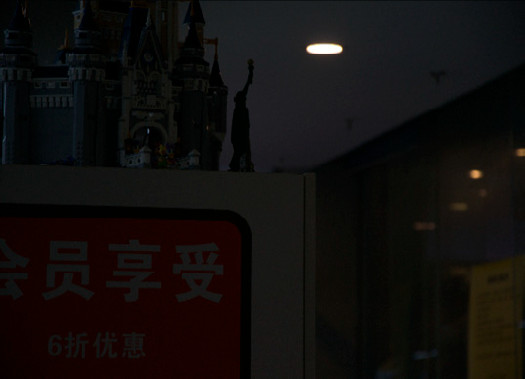
\includegraphics[width=\linewidth]{picture/LLIE/VE-LOL-L/input}
%				\captionsetup{font=scriptsize}
%				\caption*{input \\ \quad }
%				\label{fig: input}
%			\end{subfigure}
%			\begin{subfigure}{0.17\columnwidth}
%				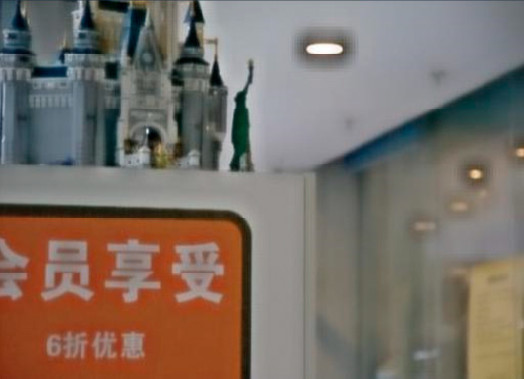
\includegraphics[width=\linewidth]{picture/LLIE/VE-LOL-L/LLNet}
%				\captionsetup{font=scriptsize}
%				\caption*{LLNet \\ (2017)}
%				\label{fig: LLNet_VE_LOL}	
%			\end{subfigure}
%			\begin{subfigure}{0.17\columnwidth}
%				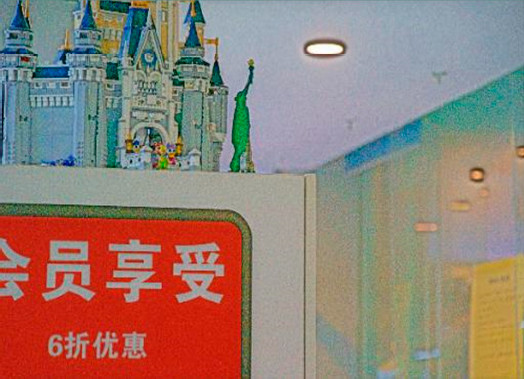
\includegraphics[width=\linewidth]{picture/LLIE/VE-LOL-L/RetinexNet}
%				\captionsetup{font=scriptsize}
%				\caption*{RetinexNet \\ (2018)}
%				\label{fig: RetinexNet_VE_LOL}	
%			\end{subfigure}
%			\begin{subfigure}{0.17\columnwidth}
%				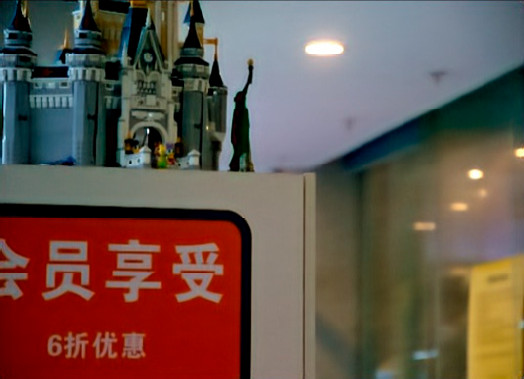
\includegraphics[width=\linewidth]{picture/LLIE/VE-LOL-L/MBLLEN}
%				\captionsetup{font=scriptsize}
%				\caption*{MBLLEN \\ (2018)}
%				\label{fig: MBLLEN_LOL}	
%			\end{subfigure}
%			\begin{subfigure}{0.17\columnwidth}
%				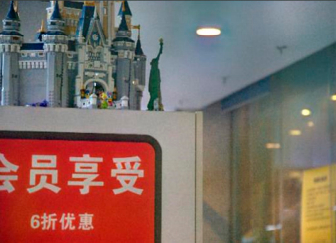
\includegraphics[width=\linewidth]{picture/LLIE/VE-LOL-L/EnlightenGAN}
%				\captionsetup{font=scriptsize}
%				\caption*{EnlightenGAN \\ (2019)}
%				\label{fig: EnlightenGAN_VE_LOL}	
%			\end{subfigure}
%			\begin{subfigure}{0.17\columnwidth}
%				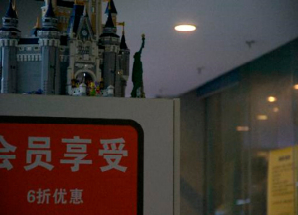
\includegraphics[width=\linewidth]{picture/LLIE/VE-LOL-L/RRDNet}
%				\captionsetup{font=scriptsize}
%				\caption*{RRDNet \\ (2020)}
%				\label{fig: RRDNet_VE_LOL}	
%			\end{subfigure}
%			\begin{subfigure}{0.17\columnwidth}
%				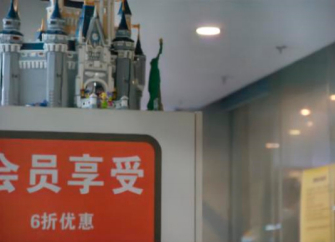
\includegraphics[width=\linewidth]{picture/LLIE/VE-LOL-L/DRBN}
%				\captionsetup{font=scriptsize}
%				\caption*{DRBN \\ (2020)}
%				\label{fig: DRBN_VE_LOL}	
%			\end{subfigure}
%			\begin{subfigure}{0.17\columnwidth}
%				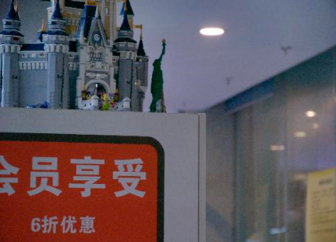
\includegraphics[width=\linewidth]{picture/LLIE/VE-LOL-L/Zero-DCE++}
%				\captionsetup{font=scriptsize}
%				\caption*{Zero-DCE++ \\ (2021)}
%				\label{fig: Zero-DCE++}	
%			\end{subfigure}
%			\begin{subfigure}{0.17\columnwidth}
%				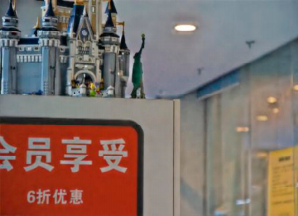
\includegraphics[width=\linewidth]{picture/LLIE/VE-LOL-L/KinD++}
%				\captionsetup{font=scriptsize}
%				\caption*{KinD++ \\ (2021)}
%				\label{fig: KinD++}	
%			\end{subfigure}
%			\begin{subfigure}{0.17\columnwidth}
%				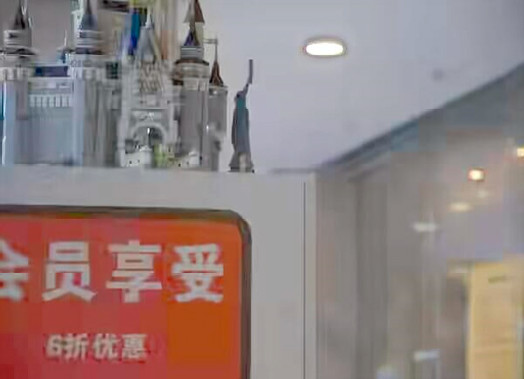
\includegraphics[width=\linewidth]{picture/LLIE/VE-LOL-L/URetinexNet}
%				\captionsetup{font=scriptsize}
%				\caption*{URetinexNet \\ (2022)}
%				\label{fig: URetinexNet}	
%			\end{subfigure}
%			\caption{
%				\label{fig: VE-LOL-L Visual} 
%				不同算法对从VE-LOL-L 数据集采样的低照度图像的可视化结果。
%			}
%		\end{figure}
		
		
		%针对极暗或极亮区域中图像边缘细节恢复的问题,一些研究者提出了在暗区域中加入敏感边缘先验的方法,以降低优化过程中的不适定性,并采用基于编码器-解码器的网络结构和回归损失来执行结构建模。进一步的研究提出了改进的模型,以解决弱光图像中局部边缘失真的问题,并对边缘图与弱恢复图的融合策略进行了优化。
		
		本研究提出了三个主要的创新点:(\textcolor{blue}{若并行架构未实现或性能不佳,则可尝试仅通过CNN分支进行图像的弱光恢复,并相应调整创新点,去除并行架构这一创新点。})
		\begin{itemize}
			\item[$\bullet$]
			%首先,提出了一种结合 CNN 和 Transformer 的并行架构用于弱光图像增强。我们发现卷积网络通过合理的增加感受野大小,可以有效捕获图像的局部特征,因而我们利用 UNet 网络对弱光图像进行弱恢复,使用 Swin Transformer 块捕获图像的长距离特征,最后通过特征融合块将二者特征加以融合。
			
			首先,提出了一种结合卷积神经网络(CNN)和Transformer的并行架构用于弱光图像增强。在该架构中,UNet网络用于捕获图像的局部特征并进行初步恢复,而Swin Transformer块用于捕获图像的长距离特征。最后,通过特征融合块将两者的特征进行融合,以实现更全面的图像增强效果。
			\item[$\bullet$] 
			%其次,在CNN分支中,提出了一个深度语义模块,融合 Swin Transformer 分支,能有效捕获图像长距离特征;
			其次,提出了一个深度语义模块,该模块融合了Swin Transformer分支,使CNN分支能够有效捕获图像的长距离特征。这种设计增强了CNN分支的能力,使其能够更好地理解图像的全局上下文信息。
			\item[$\bullet$]
			%最后,我们将深度可分离卷积融合进 CNN 分支中,应用于轻量级网络用于提取图像的局部特征;
			最后,将深度可分离卷积融合进CNN分支中,应用于轻量级网络用于提取图像的局部特征。这种设计旨在减少模型的参数量和计算复杂度,同时保持对局部特征的有效提取能力。
		\end{itemize}
		
		\section{实验计划}

		实验的过程中,确保所有的实验在相同的硬件和软件环境下进行,并且为了确保结果的可靠性,可能需要多次运行实验并取平均值。我们主要基于 PyTorch 进行模型的搭建、训练和评估。基于 scikit-image 库计算 PSNR、SSIM 等评价指标。首先构建 U-Net 基本架构模型,然后实现 Swin Transformer 块中的LocalselfAttention类,PositionEncoding类,PositionEmbedding类。

		\subsubsection{Dataset}
		
		Tab. \ref{tab: Paired_training_datases} 展示了我们在实验中会使用到的弱光数据集,这些数据集包含真实数据与合成数据。对于每个数据集,我们需要进行如下操作:
		
		\begin{itemize}
			\item [$\bullet$]
			预处理: 确保所有图像都经过相同的预处理步骤,如尺寸调整、归一化等。
			
			\item [$\bullet$]
			分割: 将每个数据集分为训练集、验证集和测试集。
		\end{itemize}
		
		\begin{table}[!htbp]
			\centering
			\tiny
			%\resizebox{\textwidth}{!}{ %按照宽度调整调整表格大小
				\begin{tabular}{>{\centering\arraybackslash}m{2.5cm}|c|c|c|c}
					
					\hline
					
					\textbf{Name} & \textbf{Number} & \textbf{Format} & \textbf{Real/Syn} & \textbf{Video} \\
					
					\hline
					
					LOL\cite{wei2018deep} & 500 & RGB & Real & \\
					
					SCIE\cite{cai2018learning} & 4,413 & RGB & Real & \\
					
					VE-LOL-L\cite{jiang2019learning} & 2,500 & RGB & Real+Syn & \\
					
					\hline
					
				\end{tabular}
				%}
			\captionsetup{font=scriptsize} %设置标题字体与表格字体一致
			\caption{\label{tab: Paired_training_datases}
				Summary of paired training datasets. 'Syn' represents Synthetic.} %表格的标题
			
		\end{table}
		
		\subsubsection{Train}
		
		\begin{itemize}
			\item [$\bullet$]
			基线模型: 首先,训练基线模型。
			
			\item [$\bullet$]
			消融研究: 接着,训练正常 BottleNeck 的模型,以进行消融实验。
		\end{itemize}
		
		\subsubsection{Performance Evaluation}
		
		对于每个数据集,使用以下指标评估模型性能:
		
		\begin{itemize}
			\item[$\bullet$]
			峰值信噪比 (PSNR)
			\item[$\bullet$]
			结构相似性指数 (SSIM)
			\item[$\bullet$]
			感知图像质量评估 (LPIPS)
		\end{itemize}
				
		\subsubsection{Loss Function}
		
		\begin{equation}
			J_{Huber}(\delta)= \frac{1}{N}\sum_{i=1}^{N}
			\left\{
			\begin{aligned}
				&\frac{1}{2}{\left\|\hat{y}_i - y_i \right\|}_2^{2}, \left\| \hat{y}_i -y_i \right\| < \delta , \\
				&\delta\left({\left\|\hat{y}_i - y_i \right\|}_1 - \frac{1}{2}\delta \right), \left\| \hat{y}_i -y_i \right\| \geq \delta.
			\end{aligned}
			\right.
			\label{eq: huber loss}
		\end{equation}
		
		\begin{equation}
			\begin{aligned}
				\ell_{feat}^{\phi,j} (\hat{y},y) = \frac{1}{C_{j}H_{j}W_{j}}{\left\| \phi_{j}(\hat{y})-\phi_{j}(y)\right\|}_{2}^2
			\end{aligned}
			\label{eq: perceptual loss}
		\end{equation}
		
		\begin{equation}
			\begin{aligned}
				\mathcal{L}^{\text{SSIM}}(P)=1-\text{SSIM}(\tilde{p}).
			\end{aligned}
			\label{eq: revised_SSIM loss}
		\end{equation}
		
		
		一共尝试以下两种损失函数的搭配方式:
		
		\begin{itemize}
			\item[$\bullet$]
			休伯损失函数和SSIM损失函数
			
			\begin{equation}
				L_{loss} = \alpha J_{Huber}(\delta) + \beta \mathcal{L}^{\text{SSIM}}(P)
			\end{equation}
			
			\item[$\bullet$]
			休伯损失函数,SSIM损失函数,Perceptual损失函数(耗费更多训练时间)
			
			\begin{equation}
				L_{loss} = \alpha J_{Huber}(\delta) + \beta \mathcal{L}^{\text{SSIM}}(P) + \gamma \ell_{feat}^{\phi,j} (\hat{y},y)
			\end{equation}
		\end{itemize}
		
	\section{实验进度}
		实现了window\_partition和window\_reverse方法,WindowAttention, PatchEmbed, PatchMerging, SwinTransformerBlock,BottleNeckBlock类
		
		
		在100Epoch下,单个SwinTransformerBlock块的情况下,未使用感知损失函数的情况下,SSIM: 0.6031,PSNR: 16.7694
		后续根据实验结果优化,增加SwinTransformerBlock块的个数,增加Embed dim,增加Epoch数量,使用感知损失函数。
		
		reshape和Embed Expanding存在区别,简单的reshape会损失特征。
	
		\renewcommand{\refname}{References}
		
		
		%	\begin{thebibliography}{00}
			
			%		\bibitem{b1}\label{cite:b1}
			%		W. Wang, C. Wei, W. Yang and J. Liu, "GLADNet: Low-Light Enhancement Network with Global Awareness," 2018 13th IEEE International Conference on Automatic Face \& Gesture Recognition (FG 2018), Xi'an, China, 2018, pp. 751-755, DOI: 10.1109/FG.2018.00118.
			
			%		\bibitem{b2}\label{cite:b2}
			%		A.\ Mahajan, K.\ Somaraj and M. Sameer, "Adopting Artificial Intelligence Powered ConvNet To Detect Epileptic Seizures," 2020 IEEE-EMBS Conference on Biomedical Engineering and Sciences (IECBES), Langkawi Island, Malaysia, 2021, pp. 427-432, DOI: 10.1109/IECBES48179.2021.9398832.
			
			%		\bibitem{Cyr}
			%		N.\ Cyr, M.\ T$\hat{e}$tu, and M.\ Breton,
			% "All-optical microwave frequency standard: a proposal,"
			%		IEEE Trans.\ Instrum.\ Meas.\ \textbf{42}, 640 (1993).
			
			
			
			%	\end{thebibliography}
		
		\bibliographystyle{unsrt}
		\bibliography{reference}
		
		
	\end{document}
